\section{Simulación del sistema con atascamiento-deslizamiento}
Se analizará la simulación de un sistema de prueba de segundo orden. Dado que la dinámica del sistema no se comprende completamente, se realizarán conclusiones que nos permitirán poder llevárnosla a nuestro caso de estudio.

\begin{equation}
G(s)=\dfrac{(0.5s+0.5)}{(s^2+2s+2)}
\end{equation}
Este sistema cuenta con dos polos y un cero.
Las representaciones gráficas ilustran de manera elocuente el efecto de la zona muerta, caracterizado por un atascamiento del sistema ante cambios en la referencia de posición. Este fenómeno desencadena una respuesta del controlador, que se traduce en un incremento del nivel de voltaje para potenciar la fuerza electromagnética. Como consecuencia, el imán experimenta un deslizamiento una vez que dicha fuerza supera los umbrales de fricción y gravedad, dando lugar al fenómeno conocido como atascamiento-deslizamiento. En esencia, la liberación del imán de la zona muerta se produce cuando estas fuerzas son sobrepasadas. En respuesta a la detección de este deslizamiento, el controlador entra en acción para restaurar la estabilidad del sistema.
\setboolean{image}{false} 
\ifthenelse{\boolean{image}}{
    \begin{figure}[htbp]
        \centering
        \subfigure[]{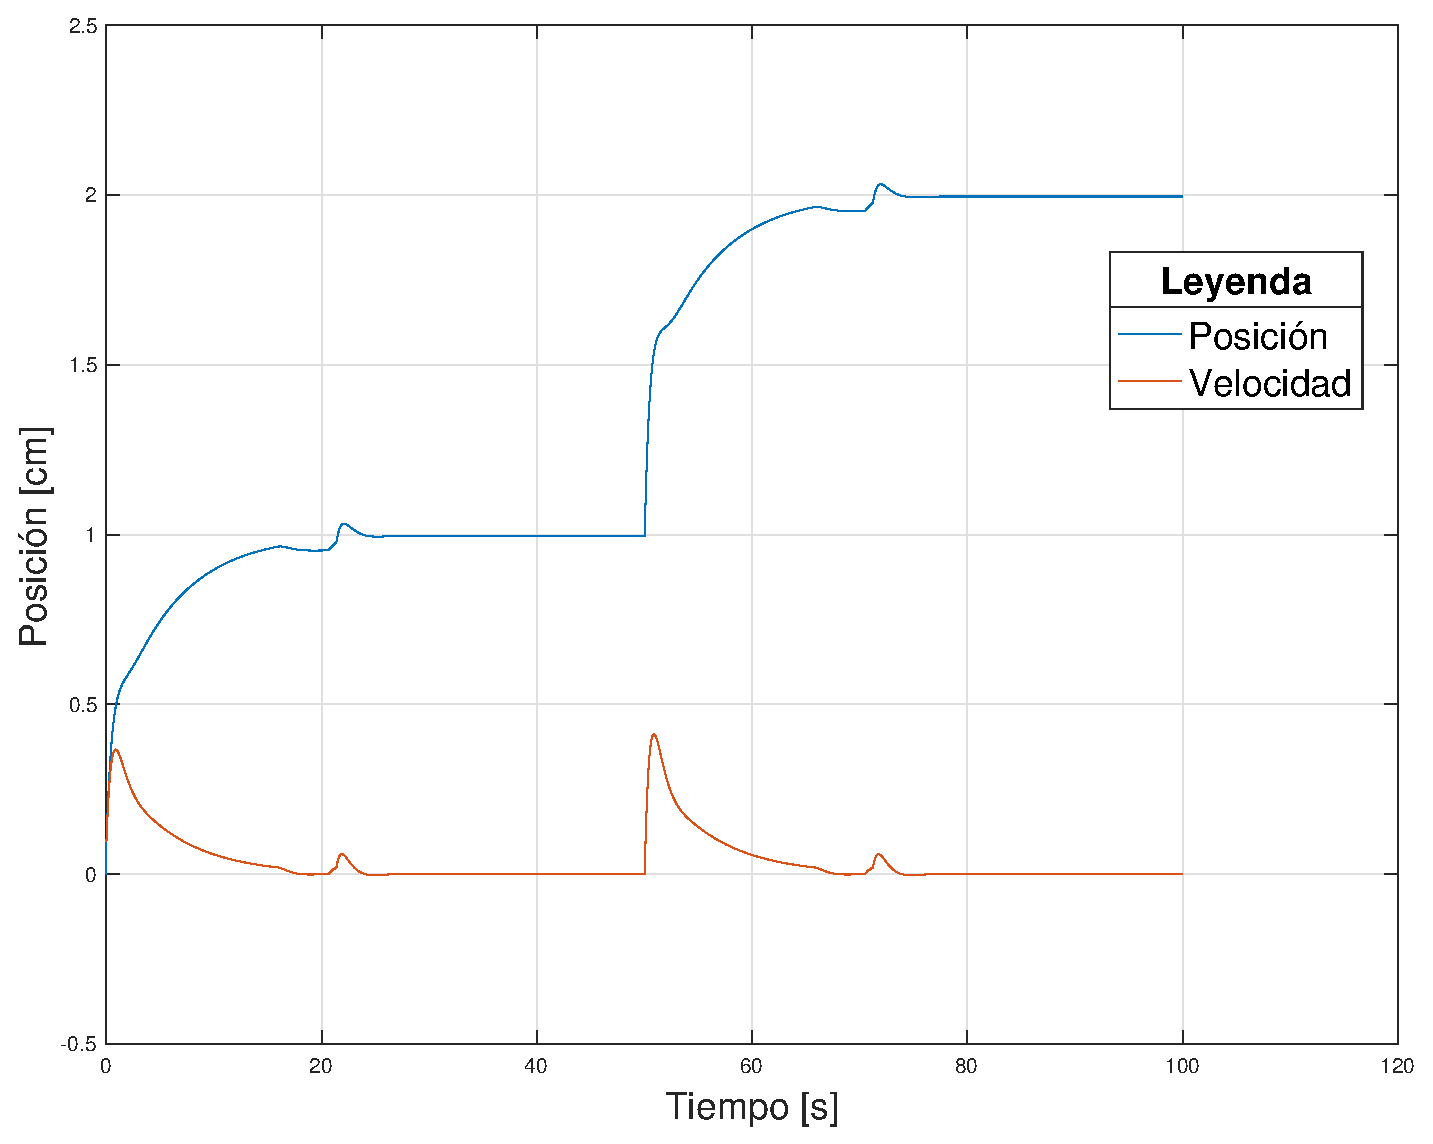
\includegraphics[width=0.45\textwidth]{images/Imagenes_De_Planta_De_Prueba/PosicionVelocidad.eps}}\hfill
        \subfigure[]{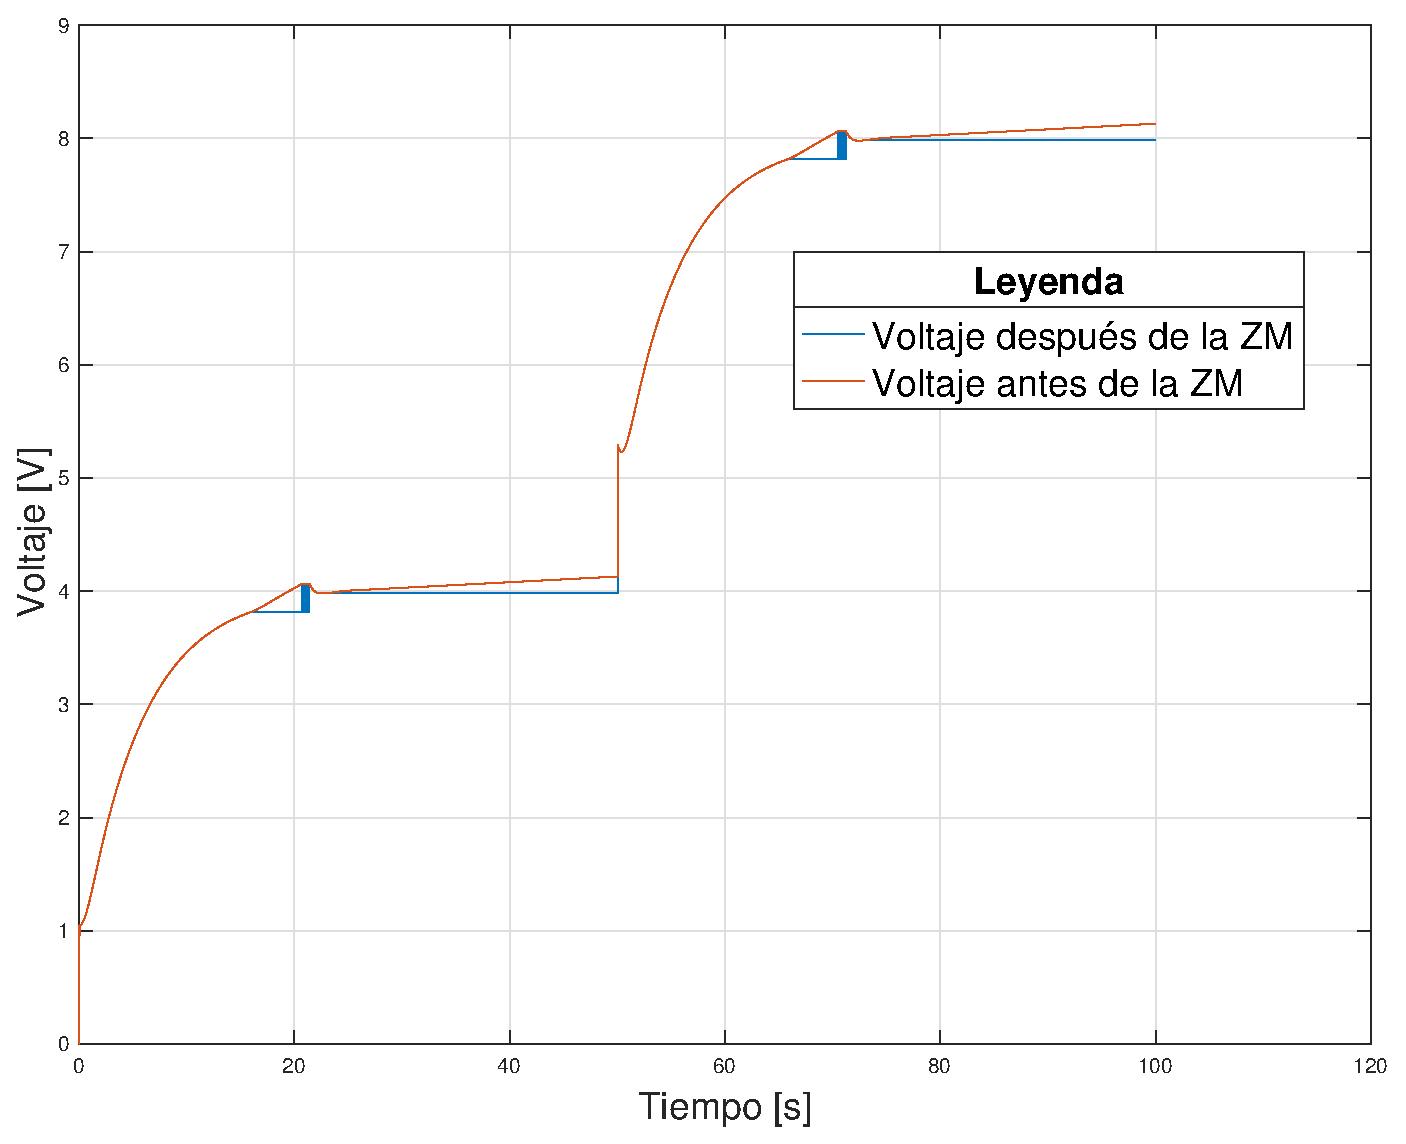
\includegraphics[width=0.45\textwidth]{images/Imagenes_De_Planta_De_Prueba/VoltajeAntesDespuesDeZM.eps}}
        \caption{(a) PosicionVelocidad (b) VoltajeAntesYDepuesDeZM}
        \label{fig:figures}
    \end{figure}
}{
    \begin{figure}[htbp]
        \centering
        \fbox{%
            \begin{minipage}[c][1in][c]{1in}
                \centering % Center the text
                Your text here
            \end{minipage}%
        }
        \caption{Planta de prueba}
        \label{fig:fbox}
    \end{figure}
}
